\documentclass[11pt]{article}

% ===================================================================
%  v7_dag_hvx_sched — explanatory document
%  Build:  cd docs && pdflatex v7_dag_hvx_sched.tex (run twice for refs)
% ===================================================================
\usepackage[margin=1in]{geometry}
\usepackage{amsmath,amssymb}
\usepackage{xcolor}
\usepackage{graphicx}
\usepackage{booktabs}
\usepackage{array}
\usepackage{tikz}
\usetikzlibrary{arrows.meta,positioning,fit,backgrounds,calc,shapes.geometric,matrix}
\usepackage{listings}
\usepackage[ruled,vlined,linesnumbered]{algorithm2e}
\usepackage{hyperref}
\hypersetup{colorlinks=true,linkcolor=blue!60!black,urlcolor=teal!60!black,citecolor=blue}
\usepackage{caption}
\captionsetup{font=small,labelfont=bf}

% ---- colors ----
\definecolor{hvxblue}{RGB}{30,90,180}
\definecolor{hvxgreen}{RGB}{20,140,70}
\definecolor{hvxred}{RGB}{200,50,40}
\definecolor{hvxgray}{RGB}{110,110,110}
\definecolor{codebg}{RGB}{248,248,245}
\definecolor{critcol}{RGB}{220,70,60}
\definecolor{workcol}{RGB}{60,120,200}

% ---- C listings style ----
\lstdefinestyle{cstyle}{
  language=C, basicstyle=\ttfamily\footnotesize, backgroundcolor=\color{codebg},
  keywordstyle=\color{hvxblue}\bfseries, commentstyle=\color{hvxgreen}\itshape,
  stringstyle=\color{hvxred}, numbers=left, numberstyle=\tiny\color{hvxgray},
  numbersep=7pt, frame=single, framesep=4pt, rulecolor=\color{gray!40},
  breaklines=true, showstringspaces=false, columns=fullflexible, tabsize=2,
  morekeywords={HVX_Vector,uint32_t,uint64_t,int32_t,size_t,inline,Matrix,restrict}
}
\lstset{style=cstyle}

\newcommand{\code}[1]{\texttt{\small #1}}
\newcommand{\file}[1]{\textcolor{hvxblue}{\texttt{#1}}}
\newcommand{\vt}{v^{\!\top}}

\title{\textbf{\code{v7\_dag\_hvx\_sched}}\\[4pt]
\large DAG-Priority HVX Scheduling for Householder QR on Hexagon v69\\[2pt]
\normalsize A code walkthrough with visuals, worked numbers, and pseudocode}
\author{QR-on-Hexagon research notes}
\date{\today}

\begin{document}
\maketitle

\begin{abstract}
\noindent
This document explains \file{v7\_dag\_hvx\_sched.c}, a parallel Householder QR
factorization for the Qualcomm Hexagon~v69 DSP. The central idea is to treat the
\emph{HVX vector contexts} (only $\sim$4 are available) as the scarce, schedulable
resource of a task DAG, and to overlap the latency-bound ``reflector'' computation of
one column with the bandwidth-bound ``trailing update'' of the others. We cover the
math, the column-major HVX kernels (including a register-only horizontal reduction),
the task graph and its critical path, the persistent thread pool with an atomic
HVX-context allocator, and the two scheduler drivers (\code{async\_prio} and the
\code{barrier} ablation reference). Each mechanism is illustrated with a diagram, a
small worked numerical example, and pseudocode tied line-by-line to the source.
All cycle counts quoted are measured on the Hexagon ISS (\code{--timing}, \code{c15:14}).
\end{abstract}

\tableofcontents
\bigskip\hrule

% ===================================================================
\section{The problem and the one-paragraph idea}
% ===================================================================
We factor a real $m\times n$ matrix $A=QR$ ($Q$ orthogonal, $R$ upper triangular) by
Householder reflections. Column $k$ produces a reflector $H_k=I-\tau_k v_k v_k^{\!\top}$
that zeroes everything below the diagonal of column $k$; applying $H_k$ to every
trailing column $j>k$ is the bulk of the work. On Hexagon the multiply--accumulate
heavy ``apply'' step wants the 32-lane HVX vector unit, but only \textbf{four} HVX
\emph{contexts} exist in 128-byte mode. So the resource we must schedule is not the
thread but the \emph{vector context}.

\paragraph{The idea.} Model the factorization as a task DAG, identify its critical
path (the chain that gates all remaining parallelism), and (i) hand the scarce HVX
contexts to the highest-priority ready tasks, while (ii) overlapping the serial
reflector computation of column $k{+}1$ with the parallel trailing updates of columns
$k{+}2,\dots,n{-}1$. The result is up to $1.29\times$ over a barrier schedule on
tall-skinny (least-squares) matrices, with the benefit growing in the number of
reflectors.

% ===================================================================
\section{Mathematical background}
% ===================================================================
For column $k$, let $x=A[k{:}m,\,k]$ be the sub-diagonal column vector. The Householder
reflector is built as
\begin{align}
\alpha &= -\operatorname{sign}(x_k)\,\lVert x\rVert_2, &
v &= x - \alpha e_1,\\
\tau &= \frac{2}{\lVert v\rVert_2^{2}} = \frac{2}{v^{\!\top} v}, &
H_k &= I - \tau\, v v^{\!\top}.
\end{align}
The sign choice avoids cancellation. Applying $H_k$ to a trailing column $a=A[:,j]$ is a
rank-1 update driven by a single dot product:
\begin{equation}
\label{eq:apply}
H_k a \;=\; a - \tau\,(v^{\!\top} a)\,v \;=\; a - w\,v,\qquad w=\tau\,(v^{\!\top}a).
\end{equation}
Equation~\eqref{eq:apply} is the computational heart of the code: one \emph{reduction}
($v^{\!\top}a$, a dot product) followed by one \emph{saxpy} ($a\mathrel{-}=w\,v$). Both
map directly onto HVX.

\paragraph{Worked numerical example (one reflector).}
Take $x=(3,4)^{\!\top}$ ($m{=}2,k{=}0$). Then $\lVert x\rVert=5$, and since $x_0=3>0$,
$\alpha=-5$. Thus $v=x-\alpha e_1=(3{-}(-5),\,4)=(8,4)$, $v^{\!\top}v=80$, $\tau=2/80=0.025$.
Apply $H_0$ to $a=(3,4)^{\!\top}$ (the pivot column itself):
\[
w=\tau\,(v^{\!\top}a)=0.025\,(8\cdot3+4\cdot4)=0.025\cdot 40 = 1.0,\quad
H_0 a = (3,4)-1.0\,(8,4)=(-5,0)^{\!\top}.
\]
The diagonal becomes $\alpha=-5$ and the sub-diagonal is annihilated, as required.

% ===================================================================
\section{Data layout and HVX in 60 seconds}
% ===================================================================
The matrix is \textbf{column-major}: \code{MAT(A,i,j) = A.data[j*m + i]}, so a whole
column is contiguous --- ideal for vector loads. We require $m$ to be a multiple of
$32$ (\code{HVX\_FLOAT\_LANES}), so each column is an exact number of HVX vectors.

\begin{figure}[h]
\centering
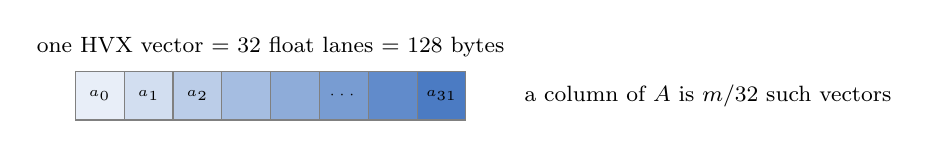
\begin{tikzpicture}[scale=0.62]
  % column-major memory strip
  \foreach \i in {0,...,7} {
    \fill[hvxblue!\the\numexpr10+10*\i\relax!white] (\i,0) rectangle (\i+1,1);
  }
  \draw[step=1,gray] (0,0) grid (8,1);
  \node at (4,1.5) {\footnotesize one HVX vector = 32 float lanes = 128 bytes};
  \foreach \i/\l in {0/$a_0$,1/$a_1$,2/$a_2$,7/$a_{31}$} \node at (\i+0.5,0.5){\tiny \l};
  \node at (5.5,0.5){\tiny $\cdots$};
  % saxpy / reduce annotation
  \node[anchor=west] at (9,0.5){\footnotesize a column of $A$ is $m/32$ such vectors};
\end{tikzpicture}
\caption{Column-major layout: a column is contiguous and tiles exactly into 32-lane
HVX vectors (because $32 \mid m$).}
\end{figure}

\paragraph{The horizontal-reduction trick (\code{hvx\_reduce\_qf32}).}
A dot product accumulates a \emph{vector} of 32 partial sums; we still need the scalar
total. The naive way stores the vector to a 32-element array and loops in scalar
($\sim$40 cycles, plus memory traffic). Instead the code does a register-only
tree reduction: rotate-and-add, halving the live partial sums each stage. Because
\code{Q6\_V\_vror\_VR} rotates by \emph{bytes} and each float is 4 bytes, halving 32
lanes uses rotates of $64,32,16,8,4$ bytes (5 stages, $\log_2 32$).

\begin{figure}[h]
\centering
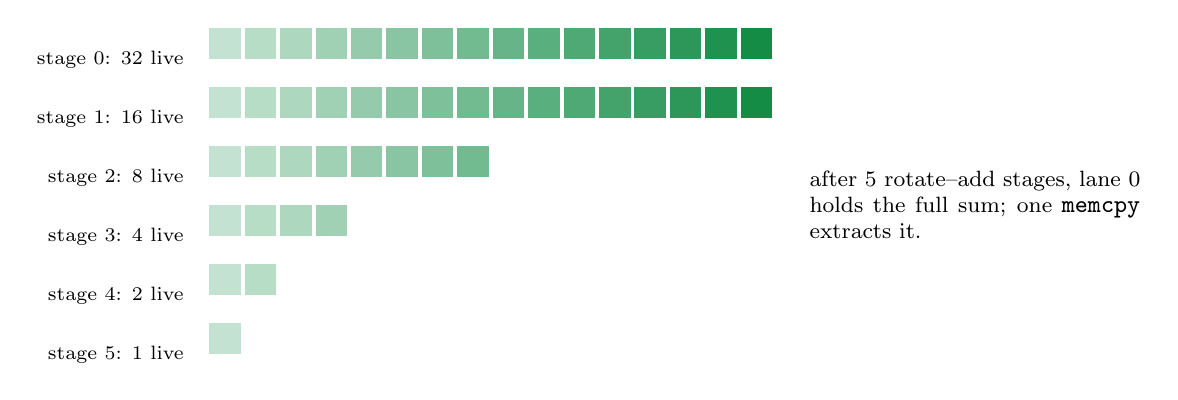
\begin{tikzpicture}[scale=0.5,every node/.style={font=\scriptsize}]
  \def\lvls{{32,16,8,4,2,1}}
  \foreach \s in {0,...,5} {
    \pgfmathparse{\lvls[\s]}\edef\w{\pgfmathresult}
    \node[anchor=east] at (-0.4,-1.5*\s) {stage \s: \w\ live};
    \foreach \b in {0,...,15} {
      \pgfmathtruncatemacro\show{ \b < \w ? 1 : 0 }
      \ifnum\show=1
        \fill[hvxgreen!\the\numexpr25+5*\b\relax!white] (\b*0.9,-1.5*\s) rectangle (\b*0.9+0.8,-1.5*\s+0.8);
      \fi
    }
  }
  \node[anchor=west,font=\footnotesize] at (15,-3.7)
    {\parbox{4.2cm}{after 5 rotate--add stages, lane~0 holds the full sum; one
     \code{memcpy} extracts it.}};
\end{tikzpicture}
\caption{Register-only tree reduction: each stage rotates the vector by half its live
width and adds, collapsing 32 partial sums into lane~0 with no memory traffic.}
\end{figure}

\begin{lstlisting}[caption={\file{hvx\_utils.h} --- the reduction and the fused dot product (verbatim).}]
static inline float hvx_reduce_qf32(HVX_Vector vqsum) {
    HVX_Vector v = Q6_Vsf_equals_Vqf32(vqsum);   /* qf32 -> sf */
    HVX_Vector vhi;
    vhi = Q6_V_vror_VR(v, 64); v = Q6_Vsf_equals_Vqf32(Q6_Vqf32_vadd_VsfVsf(v, vhi));
    vhi = Q6_V_vror_VR(v, 32); v = Q6_Vsf_equals_Vqf32(Q6_Vqf32_vadd_VsfVsf(v, vhi));
    vhi = Q6_V_vror_VR(v, 16); v = Q6_Vsf_equals_Vqf32(Q6_Vqf32_vadd_VsfVsf(v, vhi));
    vhi = Q6_V_vror_VR(v,  8); v = Q6_Vsf_equals_Vqf32(Q6_Vqf32_vadd_VsfVsf(v, vhi));
    vhi = Q6_V_vror_VR(v,  4); v = Q6_Vsf_equals_Vqf32(Q6_Vqf32_vadd_VsfVsf(v, vhi));
    float result; memcpy(&result, &v, sizeof(float));  /* lane 0 = full sum */
    return result;
}
static inline float hvx_dot_col_v(const float* col_j, const float* v, int m) {
    HVX_Vector vacc = Q6_V_vzero();
    for (int i = 0; i < m; i += HVX_FLOAT_LANES) {           /* 32 lanes / iter */
        HVX_Vector va = *(const HVX_VectorU_t*)(col_j + i);
        HVX_Vector vv = *(const HVX_VectorU_t*)(v + i);
        vacc = Q6_Vqf32_vadd_Vqf32Vqf32(vacc, Q6_Vqf32_vmpy_VsfVsf(va, vv));
    }
    return hvx_reduce_qf32(vacc);                            /* tree reduce */
}
\end{lstlisting}

\noindent The accumulation uses the \code{qf32} (``quad float'') format for an extra
guard against rounding during the long sum, converting back to IEEE \code{sf} only at
the end --- this is what keeps the result bit-comparable to the scalar reference.

% ===================================================================
\section{The trailing-column kernel: dot then saxpy}
% ===================================================================
Each trailing column update is exactly Eq.~\eqref{eq:apply}: a fused HVX dot product, a
scalar $w=\tau\cdot\text{dot}$, a broadcast (\code{vsplat}) of $w$, and a vectorized
saxpy that writes the column back.

\begin{lstlisting}[caption={\code{apply\_col\_hvx} --- update one trailing column (verbatim).}]
static inline void apply_col_hvx(Matrix* A, const float* v, float tau, int j, int m) {
    float* col_j = &MAT(*A, 0, j);
    float dot = hvx_dot_col_v(col_j, v, m);          /* v^T a  (reduction)     */
    float w = tau * dot;                             /* scalar weight          */
    HVX_Vector vw = Q6_V_vsplat_R(*(uint32_t*)&w);   /* broadcast w to 32 lanes */
    for (int i = 0; i < m; i += HVX_FLOAT_LANES) {   /* a -= w * v  (saxpy)    */
        HVX_Vector va = *(HVX_VectorU*)(col_j + i);
        HVX_Vector vv = *(const HVX_VectorU*)(v + i);
        HVX_Vector va_qf = Q6_Vqf32_vadd_VsfVsf(va, Q6_V_vzero());
        HVX_Vector vp    = Q6_Vqf32_vmpy_VsfVsf(vw, vv);
        *(HVX_VectorU*)(col_j + i) =
            Q6_Vsf_equals_Vqf32(Q6_Vqf32_vsub_Vqf32Vqf32(va_qf, vp));
    }
}
\end{lstlisting}

\noindent A scalar twin, \code{apply\_col\_scalar}, performs the identical math without
HVX; it is the fallback for worker threads that do not win a vector context (see
\S\ref{sec:alloc}). Both iterate $i$ over the \emph{full} range $[0,m)$ because
\code{compute\_reflector} zeroes $v[0{:}k]$, so the masked-out top of the column
contributes nothing --- this lets every loop stay 32-lane aligned.

% ===================================================================
\section{The task DAG and its critical path}
% ===================================================================
Define two task kinds:
\begin{itemize}\itemsep1pt
  \item $T(k,k)$ --- \textbf{compute reflector} for column $k$ (norm, $v$, $\tau$): latency-bound, scalar.
  \item $T(k,j)$, $j>k$ --- \textbf{trailing update} of column $j$ with reflector $k$: bandwidth-bound, vector.
\end{itemize}
Dependencies: $T(k,j)$ needs $T(k,k)$ (the reflector must exist --- \emph{intra-step})
and $T(k{-}1,j)$ (column $j$ must already carry the previous step's update ---
\emph{inter-step}).

\begin{figure}[h]
\centering
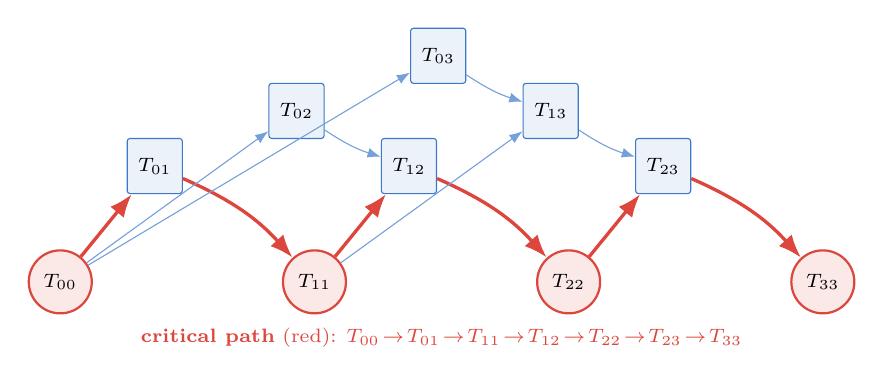
\begin{tikzpicture}[
  >=Latex, node distance=10mm and 13mm,
  reflector/.style={circle,draw=critcol,fill=critcol!12,thick,minimum size=8mm,font=\scriptsize},
  update/.style={rectangle,draw=workcol,fill=workcol!10,minimum size=7mm,font=\scriptsize,rounded corners=1pt},
  crit/.style={->,critcol,very thick},
  dep/.style={->,workcol!70,thin}]
  % reflectors on the diagonal
  \node[reflector] (r0) {$T_{00}$};
  \node[reflector,right=24mm of r0] (r1) {$T_{11}$};
  \node[reflector,right=24mm of r1] (r2) {$T_{22}$};
  \node[reflector,right=24mm of r2] (r3) {$T_{33}$};
  % updates for step 0
  \node[update,above=7mm of r0,xshift=12mm] (u01) {$T_{01}$};
  \node[update,above=14mm of r0,xshift=30mm] (u02) {$T_{02}$};
  \node[update,above=21mm of r0,xshift=48mm] (u03) {$T_{03}$};
  % updates for step 1
  \node[update,above=7mm of r1,xshift=12mm] (u12) {$T_{12}$};
  \node[update,above=14mm of r1,xshift=30mm] (u13) {$T_{13}$};
  % updates for step 2
  \node[update,above=7mm of r2,xshift=12mm] (u23) {$T_{23}$};

  % critical path: r0 -> u01 -> r1 -> u12 -> r2 -> u23 -> r3
  \draw[crit] (r0) -- (u01);
  \draw[crit] (u01) to[bend left=12] (r1);
  \draw[crit] (r1) -- (u12);
  \draw[crit] (u12) to[bend left=12] (r2);
  \draw[crit] (r2) -- (u23);
  \draw[crit] (u23) to[bend left=12] (r3);

  % intra-step (reflector -> its other updates)
  \draw[dep] (r0) -- (u02);  \draw[dep] (r0) -- (u03);
  \draw[dep] (r1) -- (u13);
  % inter-step (col j prev update -> this update)
  \draw[dep] (u02) to[bend right=8] (u12);
  \draw[dep] (u03) to[bend right=8] (u13);
  \draw[dep] (u13) to[bend right=8] (u23);

  \node[font=\scriptsize,critcol] at (current bounding box.south) [yshift=-3mm]
    {\textbf{critical path} (red): $T_{00}\!\to\!T_{01}\!\to\!T_{11}\!\to\!T_{12}\!\to\!T_{22}\!\to\!T_{23}\!\to\!T_{33}$};
\end{tikzpicture}
\caption{Task DAG for $n{=}4$. Diagonal circles are reflector tasks $T_{kk}$; squares
are trailing updates $T_{kj}$. The red critical path threads
\emph{reflector $\to$ update of the very next column $\to$ next reflector}. Blue edges
are the remaining (parallel-friendly) dependencies.}
\label{fig:dag}
\end{figure}

\paragraph{The key observation.} At step $k$ the only critical-path trailing task is the
update of \textbf{column $k{+}1$}: reflector $k{+}1$ reads column $k{+}1$, so it cannot
start until $T(k,k{+}1)$ finishes. Columns $k{+}2,\dots,n{-}1$ are not on the critical
path --- they can be updated lazily, in parallel, while we race ahead on the diagonal.
This single fact is the entire scheduling strategy:
\begin{center}\itshape
``Update column $k{+}1$ first; then compute reflector $k{+}1$ while workers finish
columns $k{+}2..n{-}1$ of step $k$.''
\end{center}
The priority of a trailing task is therefore just its (ascending) column index --- a
\emph{closed-form} critical-path priority, needing no runtime graph analysis.

% ===================================================================
\section{HVX-context allocation: the scarce resource}
\label{sec:alloc}
% ===================================================================
On v69, \code{qurt\_hvx\_get\_units()} returns \code{0x400} =
\code{QURT\_HVX\_HW\_UNITS\_4X128B\_0X64B}, i.e. \textbf{four} 128-byte contexts. With
$n_t$ worker threads only $\min(n_t,4)$ can vectorize at once; the rest must run the
scalar twin. The allocator must therefore (a) never block, and (b) deterministically
give contexts to the first (highest-priority) claimants.

\paragraph{Why not \code{qurt\_hvx\_try\_lock}?} On v65+ it is deprecated and does
\emph{not} actually grant a context --- using it silently drops \emph{every} worker to
scalar ($\sim$5$\times$ slowdown, discovered the hard way). The fix is an
\textbf{atomic budget}: a worker claims a slot with one \code{qurt\_atomic\_inc\_return};
only if its slot number is within budget does it call the (now provably free, hence
non-blocking) \code{qurt\_hvx\_lock}.

\begin{figure}[h]
\centering
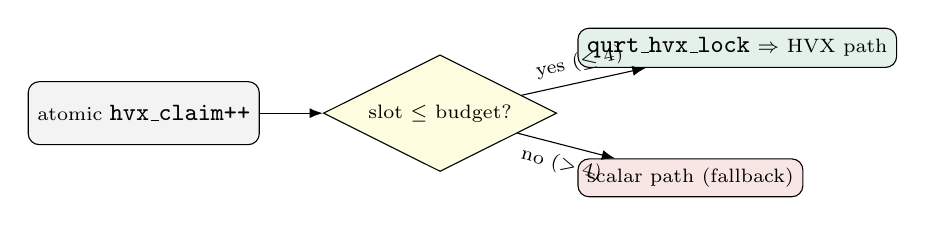
\begin{tikzpicture}[font=\scriptsize,>=Latex,node distance=4mm]
  \node[draw,rounded corners,fill=hvxgray!8,minimum width=2.1cm,minimum height=8mm] (claim) {atomic \code{hvx\_claim++}};
  \node[draw,diamond,aspect=2,fill=yellow!12,right=8mm of claim,minimum width=2.4cm] (test) {slot $\le$ budget?};
  \node[draw,rounded corners,fill=hvxgreen!12,above right=2mm and 10mm of test,minimum width=2.6cm] (hvx) {\code{qurt\_hvx\_lock} $\Rightarrow$ HVX path};
  \node[draw,rounded corners,fill=hvxred!12,below right=2mm and 10mm of test,minimum width=2.6cm] (sca) {scalar path (fallback)};
  \draw[->] (claim) -- (test);
  \draw[->] (test) -- node[above,sloped]{yes ($\le 4$)} (hvx);
  \draw[->] (test) -- node[below,sloped]{no ($>4$)} (sca);
\end{tikzpicture}
\caption{Per-dispatch HVX-context allocation. The atomic counter makes the decision
race-free and the \code{qurt\_hvx\_lock} call is only reached when a context is provably
available.}
\end{figure}

\begin{lstlisting}[caption={\code{pool\_do\_col\_hh} --- worker body: ascending-column claim, budgeted HVX, publish completion.}]
static void pool_do_col_hh(void) {
    Matrix* A = g_pool.hh_A; int m = A->m, chunk = g_pool.hh_chunk_size;
    const float* v = g_pool.hh_v; float tau = g_pool.hh_tau;
    int got_hvx = 0;                                  /* 0 unclaimed, 1 HVX, -1 scalar */
    while (1) {
        unsigned int ci = qurt_atomic_inc_return(&g_pool.hh_counter) - 1;   /* ascending */
        int col_base = g_pool.hh_col_start + (int)ci * chunk;
        if (col_base >= g_pool.hh_col_end) break;
        int col_end_c = col_base + chunk;
        if (col_end_c > g_pool.hh_col_end) col_end_c = g_pool.hh_col_end;
        if (got_hvx == 0) {                            /* claim a context once */
            unsigned int slot = qurt_atomic_inc_return(&g_pool.hvx_claim);
            if ((int)slot <= g_pool.hvx_worker_units &&
                qurt_hvx_lock(QURT_HVX_MODE_128B) == QURT_EOK) got_hvx = 1;
            else got_hvx = -1;                         /* over budget -> scalar */
        }
        for (int j = col_base; j < col_end_c; j++) {
            if (got_hvx == 1) apply_col_hvx(A, v, tau, j, m);
            else              apply_col_scalar(A, v, tau, j, m);
            __asm__ __volatile__("" ::: "memory");     /* publish data before flag */
            g_pool.col_done[j] = 1;                    /* lets the driver advance */
        }
    }
    if (got_hvx == 1) qurt_hvx_unlock();
}
\end{lstlisting}

% ===================================================================
\section{The persistent thread pool}
% ===================================================================
Spawning a thread per Householder step is far too expensive ($\sim$30--40k cycles each).
Instead $n_t$ workers are created \emph{once} and parked on per-worker QuRT signals.
A dispatch is a signal-set; completion is an atomic counter that, on reaching zero,
sets a master signal the driver waits on.

\begin{figure}[h]
\centering
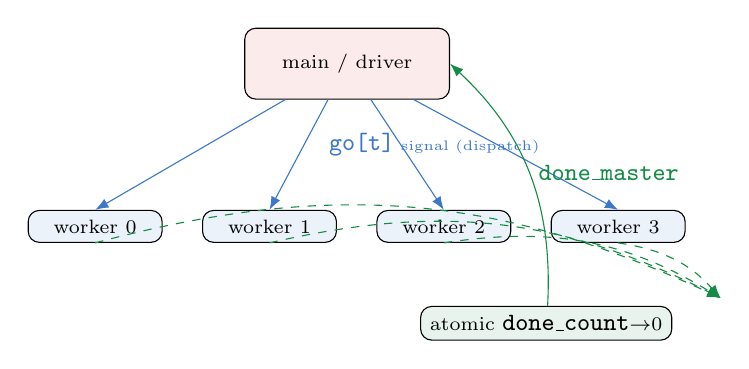
\begin{tikzpicture}[font=\scriptsize,>=Latex,node distance=6mm]
  \node[draw,rounded corners,fill=critcol!10,minimum width=2.6cm,minimum height=9mm] (main) {main / driver};
  \node[draw,rounded corners,fill=workcol!10,below=14mm of main,xshift=-3.2cm,minimum width=1.7cm] (w0){worker 0};
  \node[draw,rounded corners,fill=workcol!10,right=5mm of w0,minimum width=1.7cm] (w1){worker 1};
  \node[draw,rounded corners,fill=workcol!10,right=5mm of w1,minimum width=1.7cm] (w2){worker 2};
  \node[draw,rounded corners,fill=workcol!10,right=5mm of w2,minimum width=1.7cm] (w3){worker 3};
  \foreach \w in {w0,w1,w2,w3} \draw[->,workcol] (main) -- node[sloped,above,font=\tiny]{} (\w.north);
  \node[font=\tiny,workcol] at ($(main)!0.5!(w1)$) [xshift=1.6cm]{\code{go[t]} signal (dispatch)};
  \foreach \w in {w0,w1,w2,w3} \draw[->,hvxgreen,dashed] (\w.south) to[bend left=20] ($(w3.south)+(1.3,-0.7)$);
  \node[draw,rounded corners,fill=hvxgreen!10,below=8mm of w2,xshift=1.3cm,minimum width=3cm] (done){atomic \code{done\_count}$\to$0};
  \draw[->,hvxgreen] (done) to[bend right=25] node[right,font=\tiny]{\code{done\_master}} (main.east);
\end{tikzpicture}
\caption{Persistent pool: the driver sets each worker's \code{go} signal; the last
worker to finish (atomic \code{done\_count} hits 0) sets \code{done\_master}, waking the
driver. No per-step thread creation.}
\end{figure}

% ===================================================================
\section{The two schedulers}
% ===================================================================

\subsection{\code{barrier} --- the ablation reference}
The straightforward schedule: compute reflector $k$, dispatch \emph{all} trailing
updates $k{+}1..n{-}1$, wait for every one (a barrier), then move to $k{+}1$. This is
the baseline behavior; it is correct but leaves the reflector computation strictly
serial between parallel bursts.

\begin{algorithm}[H]
\caption{\code{qr\_dag\_barrier} (reference; no overlap)}
\SetKwInOut{In}{input}
\For{$k \gets 0$ \KwTo $n-1$}{
  $(\alpha,\tau,v) \gets$ \texttt{compute\_reflector}$(A,k)$\;
  \texttt{dispatch} trailing updates for columns $[k{+}1, n)$\;
  \texttt{wait\_done}\tcp*{full barrier: all of step $k$ finishes}
  $A[k,k]\gets\alpha$;\quad zero $A[k{+}1{:}m,\,k]$\;
}
\end{algorithm}

\subsection{\code{async\_prio} --- critical-path pivot overlap}
The optimized schedule exploits Fig.~\ref{fig:dag}. The driver itself executes the
\emph{critical} column $k{+}1$ on a briefly-held HVX context (between the previous join
and this dispatch, when no worker is active), dispatches only the \emph{non-critical}
columns $[k{+}2,n)$ to the workers, and then computes reflector $k{+}1$
\textbf{in parallel} with those workers. Double-buffered reflectors (\code{vbuf[2]})
let step $k$'s $v$ stay live while step $k{+}1$'s $v$ is built.

\begin{algorithm}[H]
\caption{\code{qr\_dag\_async\_prio} (critical-path overlap)}
$(\alpha_{\mathrm{cur}},\tau_{\mathrm{cur}},v_{\mathrm{cur}}) \gets$ \texttt{compute\_reflector}$(A,0)$\;
\For{$k \gets 0$ \KwTo $n-1$}{
  \tcp{critical task $T(k,k{+}1)$: driver does it now, on HVX}
  \If{$k{+}1<n$}{ briefly lock HVX; \texttt{apply\_col}$(A,v_{\mathrm{cur}},\tau_{\mathrm{cur}},k{+}1)$; unlock\;}
  \tcp{non-critical columns go to the workers (all contexts)}
  \texttt{dispatch\_nonblocking}$(A,v_{\mathrm{cur}},\tau_{\mathrm{cur}},\,[k{+}2,n))$\;
  \tcp{overlap: build next reflector while workers run}
  \If{$k{+}1<n$}{ $(\alpha_{\mathrm{nxt}},\tau_{\mathrm{nxt}},v_{\mathrm{nxt}}) \gets$ \texttt{compute\_reflector}$(A,k{+}1)$\;}
  \texttt{wait\_done}\tcp*{join workers for $[k{+}2,n)$}
  $A[k,k]\gets\alpha_{\mathrm{cur}}$;\quad zero $A[k{+}1{:}m,\,k]$\;
  swap (cur, nxt)\;
}
\end{algorithm}

\paragraph{Why not just spin on \code{col\_done[k+1]}?} The first implementation had the
driver busy-wait until the workers flagged column $k{+}1$ done, then compute the next
reflector. On an in-order SMT DSP a spinning thread \emph{steals} a hardware thread slot
and memory bandwidth from the HVX workers --- measured $\sim$5$\times$ slowdown. The cure
is to give the driver \emph{real work} (the critical column) rather than a spin loop.

\begin{figure}[h]
\centering
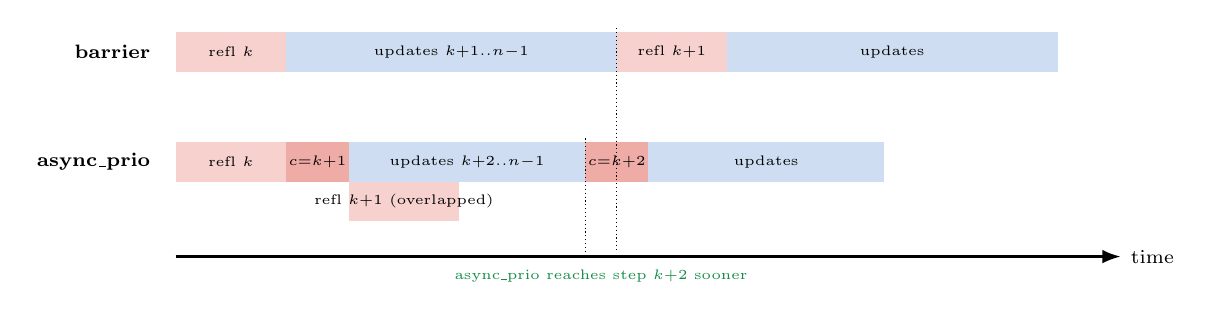
\begin{tikzpicture}[font=\scriptsize,>=Latex]
  % timeline axis
  \def\tw{12}
  % --- barrier ---
  \node[anchor=east] at (-0.2,0) {\textbf{barrier}};
  \fill[critcol!25] (0,-0.25) rectangle (1.4,0.25); \node at (0.7,0){\tiny refl $k$};
  \fill[workcol!25] (1.4,-0.25) rectangle (5.6,0.25); \node at (3.5,0){\tiny updates $k{+}1..n{-}1$};
  \fill[critcol!25] (5.6,-0.25) rectangle (7.0,0.25); \node at (6.3,0){\tiny refl $k{+}1$};
  \fill[workcol!25] (7.0,-0.25) rectangle (11.2,0.25); \node at (9.1,0){\tiny updates};
  % --- async_prio ---
  \node[anchor=east] at (-0.2,-1.4) {\textbf{async\_prio}};
  \fill[critcol!25] (0,-1.65) rectangle (1.4,-1.15); \node at (0.7,-1.4){\tiny refl $k$};
  \fill[critcol!45] (1.4,-1.65) rectangle (2.2,-1.15); \node at (1.8,-1.4){\tiny $c{=}k{+}1$};
  \fill[workcol!25] (2.2,-1.65) rectangle (5.2,-1.15); \node at (3.7,-1.4){\tiny updates $k{+}2..n{-}1$};
  \fill[critcol!25] (2.2,-2.15) rectangle (3.6,-1.65); \node at (2.9,-1.9){\tiny refl $k{+}1$ (overlapped)};
  \fill[critcol!45] (5.2,-1.65) rectangle (6.0,-1.15); \node at (5.6,-1.4){\tiny $c{=}k{+}2$};
  \fill[workcol!25] (6.0,-1.65) rectangle (9.0,-1.15); \node at (7.5,-1.4){\tiny updates};
  \draw[->,thick] (0,-2.6) -- (\tw,-2.6) node[right]{time};
  \draw[densely dotted] (5.6,0.3) -- (5.6,-2.55);
  \draw[densely dotted] (5.2,-1.1) -- (5.2,-2.55);
  \node[hvxgreen,font=\tiny] at (5.4,-2.85) {async\_prio reaches step $k{+}2$ sooner};
\end{tikzpicture}
\caption{Schedule comparison. In \code{barrier} the reflector computations (red) are
serial gaps between parallel update bursts (blue). In \code{async\_prio} the next
reflector is computed \emph{underneath} the workers' updates, and the critical column is
done first --- shrinking the per-step critical path.}
\end{figure}

% ===================================================================
\section{Numerical / performance results}
% ===================================================================
All measured on the Hexagon ISS (\code{hexagon-sim --timing}, cycle counter
\code{c15:14}), $n_t{=}4$, deterministic test matrix. Correctness is checked against a
scalar CPU Householder ($\lvert R\rvert$ agreement and sub-diagonal residual).

\begin{table}[h]
\centering
\caption{Square matrices: where the speedup comes from (cycles, lower is better).
The \emph{policy} comparison (barrier vs.\ async\_prio, identical kernels) is a wash;
the HVX horizontal reduction dominates the gain over the \code{v0} pool baseline.}
\begin{tabular}{lrr}
\toprule
variant / mode & $128\times128$ & $256\times256$ \\
\midrule
\code{v0\_pool} (scalar reduction) & 341{,}377 & 938{,}095 \\
\code{v1} (+HVX tree reduction)    & 301{,}989 & 792{,}991 \\
\code{v7} barrier                   & 287{,}766 & 735{,}121 \\
\code{v7} async\_prio               & 289{,}327 & 724{,}195 \\
\midrule
\textit{reduction share of v7-vs-v0 gain} & $73.5\%$ & $67.8\%$ \\
\textit{pure policy (barrier vs prio)}    & $+0.5\%$ & $-1.5\%$ \\
\bottomrule
\end{tabular}
\end{table}

\begin{table}[h]
\centering
\caption{Tall-skinny matrices: here the \emph{scheduling policy} pays off. Identical
kernels; only the schedule differs. The benefit grows with $n$ (more reflectors to
overlap), not with aspect ratio.}
\begin{tabular}{lrrr}
\toprule
shape ($m\times n$) & async\_prio & barrier & barrier\,/\,async\_prio \\
\midrule
$1024\times16$ & 268{,}663 & 303{,}529 & $1.13\times$ \\
$1024\times32$ & 430{,}811 & 514{,}201 & $1.19\times$ \\
$1024\times64$ & 658{,}439 & 846{,}695 & $\mathbf{1.29\times}$ \\
$2048\times16$ & 483{,}751 & 548{,}827 & $1.13\times$ \\
$2048\times32$ & 772{,}987 & 953{,}679 & $1.23\times$ \\
$4096\times16$ & 919{,}137 & 1{,}033{,}437 & $1.12\times$ \\
$640\times64$  & 474{,}969 & 565{,}503 & $1.19\times$ \\
\bottomrule
\end{tabular}
\end{table}

\paragraph{Reading the results.}
\begin{enumerate}\itemsep1pt
\item The single biggest lever is the \textbf{register-only horizontal reduction}
($\sim$70\% of the square-matrix gain) --- a kernel optimization, not scheduling.
\item \textbf{Critical-path scheduling} is shape-conditioned: neutral on square
matrices but worth up to $1.29\times$ on tall-skinny ones, precisely the
overdetermined least-squares regime. The win scales in $n$: at $m{=}1024$,
$n{=}16/32/64 \Rightarrow 1.13/1.19/1.29\times$, because more columns means more
reflector computations to hide under the trailing updates.
\item The \textbf{HVX context}, not the thread, is the binding resource: beyond
4 threads the surplus workers fall to scalar, so context-aware budgeting (not adding
threads) is what preserves scaling.
\end{enumerate}

% ===================================================================
\section{End-to-end control flow}
% ===================================================================
\begin{algorithm}[H]
\caption{\code{main} (driver glue)}
read \code{inparams.txt}: $m,n,n_t,\text{chunk},\text{sched},\text{nb}$\;
\texttt{create\_matrix}; \texttt{fill\_test\_matrix}\;
run scalar CPU Householder reference (timed)\;
\texttt{pool\_init}$(n_t)$\tcp*{spawn workers once}
\texttt{get\_cycles} $\to t_2$\;
\eIf{\textnormal{sched} $=$ \textnormal{BARRIER}}{\texttt{qr\_dag\_barrier}$(A)$\;}{\texttt{qr\_dag\_async\_prio}$(A)$\;}
\texttt{get\_cycles} $\to t_3$;\quad \texttt{pool\_shutdown}\;
verify $\lvert R\rvert$ vs reference; report cycles $t_3{-}t_2$, error, sub-diagonal residual\;
\end{algorithm}

\paragraph{Build \& run.} The variant is built and simulated through the project
Makefile:
\begin{center}
\code{make v7\_dag\_hvx\_sched}\quad then\quad \code{make sim-v7\_dag\_hvx\_sched}
\end{center}
with \code{build/inparams.txt} holding \code{m n nt chunk sched nb}
(\code{sched}: 0 = \code{async\_prio}, 1 = \code{barrier}).

% ===================================================================
\section{Appendix: complete pseudocode}
% ===================================================================
This appendix gives pseudocode for \emph{every} routine in
\file{v7\_dag\_hvx\_sched.c}, in dependency order, faithful to the source. Shared
state of the thread pool is the global record $g$ (fields named as in the C
\code{ThreadPool} struct).

\subsection{HVX numeric helpers (\file{hvx\_utils.h})}

\begin{algorithm}[H]
\caption{\textsc{HvxReduceQf32}$(\mathbf{s})$ --- horizontal sum of a 32-lane accumulator}
\KwIn{$\mathbf{s}$: 32-lane \code{qf32} vector of partial sums}
\KwOut{scalar $\sum_{\ell} \mathbf{s}[\ell]$}
$\mathbf{v} \gets \textsc{qf32\_to\_sf}(\mathbf{s})$\;
\For{$r \in \langle 64,32,16,8,4\rangle$ \textnormal{(byte rotates; $\log_2 32 = 5$ stages)}}{
  $\mathbf{h} \gets \textsc{RotateBytes}(\mathbf{v}, r)$\;
  $\mathbf{v} \gets \textsc{qf32\_to\_sf}\big(\mathbf{v} \boxplus \mathbf{h}\big)$ \tcp*{lanewise qf32 add}
}
\Return $\mathbf{v}[0]$ \tcp*{lane 0 now holds the full sum}
\end{algorithm}

\begin{algorithm}[H]
\caption{\textsc{HvxDotColV}$(a, v, m)$ --- vectorized dot product $\vt a$}
$\mathbf{acc} \gets \mathbf{0}$ \tcp*{32-lane qf32 accumulator}
\For{$i \gets 0$ \KwTo $m-1$ \textbf{step} $32$}{
  $\mathbf{acc} \gets \mathbf{acc} \boxplus \big(\textsc{load}_{32}(a{+}i) \boxtimes \textsc{load}_{32}(v{+}i)\big)$ \tcp*{qf32 fma}
}
\Return \textsc{HvxReduceQf32}$(\mathbf{acc})$\;
\end{algorithm}

\begin{algorithm}[H]
\caption{\textsc{HvxColNormSq}$(c, m, k_{\mathrm{start}})$ --- $\lVert c[k_{\mathrm{start}}{:}m]\rVert^2$}
$\mathbf{acc} \gets \mathbf{0}$\;
\For{$i \gets k_{\mathrm{start}}$ \KwTo $m-1$ \textbf{step} $32$}{
  $\mathbf{acc} \gets \mathbf{acc} \boxplus \big(\textsc{load}_{32}(c{+}i)\big)^{\boxtimes 2}$\;
}
\Return \textsc{HvxReduceQf32}$(\mathbf{acc})$ \tcp*{requires $32 \mid k_{\mathrm{start}}$}
\end{algorithm}

\subsection{Trailing-column update kernels}

\begin{algorithm}[H]
\caption{\textsc{ApplyColHvx}$(A, v, \tau, j, m)$ --- $A[:,j] \mathrel{-}= \tau(\vt A[:,j])\,v$}
$a \gets \&A[0,j]$ \tcp*{column $j$ is contiguous (column-major)}
$\text{dot} \gets \textsc{HvxDotColV}(a, v, m)$;\quad $w \gets \tau\cdot\text{dot}$\;
$\mathbf{w} \gets \textsc{Splat}(w)$ \tcp*{broadcast scalar to 32 lanes}
\For{$i \gets 0$ \KwTo $m-1$ \textbf{step} $32$}{
  $\textsc{store}_{32}\big(a{+}i,\; \textsc{load}_{32}(a{+}i) \boxminus (\mathbf{w} \boxtimes \textsc{load}_{32}(v{+}i))\big)$\;
}
\end{algorithm}

\begin{algorithm}[H]
\caption{\textsc{ApplyColScalar}$(A, v, \tau, j, m)$ --- identical math, no HVX (fallback)}
$a \gets \&A[0,j]$;\quad $\text{dot} \gets \sum_{i=0}^{m-1} v[i]\,a[i]$;\quad $w \gets \tau\cdot\text{dot}$\;
\lForEach{$i \in [0,m)$}{$a[i] \mathrel{-}= w\,v[i]$}
\end{algorithm}

\subsection{Reflector computation}

\begin{algorithm}[H]
\caption{\textsc{ComputeReflector}$(A, m, k) \to (\alpha, \tau, v, \mathrm{valid})$}
$\mathrm{nxsq} \gets \sum_{i=k}^{m-1} A[i,k]^2$;\quad $\mathrm{nx} \gets \sqrt{\mathrm{nxsq}}$\;
\lIf{$\mathrm{nx} < 10^{-7}$}{\Return $(\cdot,0,\cdot,\mathbf{false})$ \tcp*[f]{column already zero}}
$\alpha \gets -\operatorname{sign}(A[k,k])\cdot \mathrm{nx}$\;
$v[0{:}k] \gets 0$;\quad $v[k{:}m] \gets A[k{:}m,\,k]$;\quad $v[k] \mathrel{-}= \alpha$\;
$\mathrm{nvsq} \gets \sum_{i=k}^{m-1} v[i]^2$\;
\lIf{$\mathrm{nvsq} < 10^{-10}$}{\Return $(\cdot,0,\cdot,\mathbf{false})$}
\Return $(\alpha,\; 2/\mathrm{nvsq},\; v,\; \mathbf{true})$ \tcp*{$v[0{:}k]{=}0$ lets kernels run over $[0,m)$}
\end{algorithm}

\subsection{Persistent thread pool}

\begin{algorithm}[H]
\caption{\textsc{PoolInit}$(n_t)$}
clamp $n_t$ to $[1, \textsc{MaxThreads}]$;\quad $g.n_t \gets n_t$;\quad $g.\mathrm{kind} \gets \textsc{None}$\;
\textsc{SignalInit}$(g.\mathrm{done\_master})$;\quad \lForEach{$t \in [0,n_t)$}{\textsc{SignalInit}$(g.\mathrm{go}[t])$}
\For{$t \gets 0$ \KwTo $n_t-1$}{ create worker thread running \textsc{PoolWorker}$(t)$ on a preallocated stack\;}
$g.\mathrm{running} \gets \mathbf{true}$\;
\end{algorithm}

\begin{algorithm}[H]
\caption{\textsc{PoolWorker}$(\mathrm{tid})$ --- runs for the program's lifetime}
\While{\textbf{true}}{
  \textsc{SignalWait}$(g.\mathrm{go}[\mathrm{tid}])$;\quad \textsc{SignalClear}$(g.\mathrm{go}[\mathrm{tid}])$\;
  \lIf{$g.\mathrm{kind} = \textsc{Shutdown}$}{\textbf{break}}
  \lIf{$g.\mathrm{kind} = \textsc{ColHH}$}{\textsc{PoolDoColHH}$()$}
  $r \gets \textsc{AtomicDec}(g.\mathrm{done\_count})$\;
  \lIf{$r = 0$}{\textsc{SignalSet}$(g.\mathrm{done\_master})$ \tcp*[f]{last one out wakes the driver}}
}
\end{algorithm}

\begin{algorithm}[H]
\caption{\textsc{PoolDoColHH}$()$ --- worker body: ascending claim, budgeted HVX, publish}
$\mathrm{got} \gets 0$ \tcp*{0 unclaimed, $1$ holds HVX context, $-1$ scalar}
\While{\textbf{true}}{
  $\mathrm{ci} \gets \textsc{AtomicInc}(g.\mathrm{hh\_counter}) - 1$ \tcp*{ascending = priority order}
  $\mathrm{base} \gets g.\mathrm{hh\_col\_start} + \mathrm{ci}\cdot g.\mathrm{chunk}$\;
  \lIf{$\mathrm{base} \ge g.\mathrm{hh\_col\_end}$}{\textbf{break}}
  $\mathrm{end} \gets \min(\mathrm{base}+g.\mathrm{chunk},\; g.\mathrm{hh\_col\_end})$\;
  \If{$\mathrm{got} = 0$}{
    $\mathrm{slot} \gets \textsc{AtomicInc}(g.\mathrm{hvx\_claim})$\;
    \eIf{$\mathrm{slot} \le g.\mathrm{hvx\_worker\_units}$ \textbf{and} \textsc{HvxLock}$()$ succeeds}{$\mathrm{got} \gets 1$}{$\mathrm{got} \gets -1$ \tcp*[f]{over budget $\Rightarrow$ scalar}}
  }
  \For{$j \gets \mathrm{base}$ \KwTo $\mathrm{end}-1$}{
    \leIf{$\mathrm{got}=1$}{\textsc{ApplyColHvx}$(g.A, g.v, g.\tau, j, m)$}{\textsc{ApplyColScalar}$(\cdots)$}
    \textsc{MemoryBarrier}$()$;\quad $g.\mathrm{col\_done}[j] \gets 1$ \tcp*{publish for the driver}
  }
}
\lIf{$\mathrm{got}=1$}{\textsc{HvxUnlock}$()$}
\end{algorithm}

\begin{algorithm}[H]
\caption{\textsc{PoolDispatchNonblocking}$(A, v, \tau, c_s, c_e, \mathrm{chunk}) \to \mathrm{dispatched}$}
\lIf{$c_e \le c_s$ \textbf{or} $\lnot g.\mathrm{running}$}{\Return $0$}
\lForEach{$j \in [c_s, c_e)$}{$g.\mathrm{col\_done}[j] \gets 0$}
set job descriptor: $g.\{\mathrm{kind}{=}\textsc{ColHH}, A, v, \tau, \mathrm{hh\_col\_start}{=}c_s, \mathrm{hh\_col\_end}{=}c_e, \mathrm{chunk}\}$\;
$g.\mathrm{hh\_counter} \gets 0$;\quad $g.\mathrm{hvx\_claim} \gets 0$;\quad $g.\mathrm{done\_count} \gets g.n_t$\;
\textsc{SignalClear}$(g.\mathrm{done\_master})$;\quad \lForEach{$t \in [0,n_t)$}{\textsc{SignalSet}$(g.\mathrm{go}[t])$}
\Return $1$ \tcp*{returns immediately; workers now running}
\end{algorithm}

\begin{algorithm}[H]
\caption{\textsc{PoolWaitDone}$()$ and \textsc{PoolShutdown}$()$}
\textbf{PoolWaitDone:} \textsc{SignalWait}$(g.\mathrm{done\_master})$\;
\smallskip
\textbf{PoolShutdown:} $g.\mathrm{kind} \gets \textsc{Shutdown}$;\quad $g.\mathrm{done\_count} \gets g.n_t$;\quad signal every \code{go}; join all workers; destroy signals\;
\end{algorithm}

\subsection{Schedulers (drivers)}

\begin{algorithm}[H]
\caption{\textsc{QrDagBarrier}$(A)$ --- reference schedule (no overlap)}
$g.\mathrm{hvx\_worker\_units} \gets \textsc{HvxUnits}$ \tcp*{workers may use all 4 contexts}
\For{$k \gets 0$ \KwTo $n-1$}{
  $(\alpha,\tau,v,\mathrm{ok}) \gets \textsc{ComputeReflector}(A,m,k)$;\quad \lIf{$\lnot\mathrm{ok}$}{\textbf{continue}}
  $d \gets \textsc{PoolDispatchNonblocking}(A,v,\tau,\,k{+}1,\,n,\,\mathrm{chunk})$\;
  \lIf{$d$}{\textsc{PoolWaitDone}$()$ \tcp*[f]{full barrier on step $k$}}
  $A[k,k] \gets \alpha$;\quad $A[k{+}1{:}m,\,k] \gets 0$\;
}
\end{algorithm}

\begin{algorithm}[H]
\caption{\textsc{QrDagAsyncPrio}$(A)$ --- critical-path pivot overlap (the contribution)}
$g.\mathrm{hvx\_worker\_units} \gets \textsc{HvxUnits}$\;
allocate double buffers $v_{\mathrm{buf}}[0..1]$;\quad $\mathrm{cur} \gets 0$\;
$(\alpha_{\mathrm{cur}},\tau_{\mathrm{cur}},v_{\mathrm{cur}},\mathrm{valid}_{\mathrm{cur}}) \gets \textsc{ComputeReflector}(A,m,0)$\;
\For{$k \gets 0$ \KwTo $n-1$}{
  $\mathrm{nxt} \gets \mathrm{cur} \oplus 1$;\quad $d \gets 0$\;
  \tcp{(1) critical task $T(k,k{+}1)$: driver does it now, briefly on HVX}
  \If{$\mathrm{valid}_{\mathrm{cur}}$ \textbf{and} $k{+}1 < n$}{
    \leIf{\textsc{HvxLock}$()$ succeeds}{\textsc{ApplyColHvx}$(A,v_{\mathrm{cur}},\tau_{\mathrm{cur}},k{+}1,m)$; \textsc{HvxUnlock}$()$}{\textsc{ApplyColScalar}$(\cdots)$}
  }
  \tcp{(2) hand the non-critical columns to the workers (all contexts)}
  \lIf{$\mathrm{valid}_{\mathrm{cur}}$}{$d \gets \textsc{PoolDispatchNonblocking}(A,v_{\mathrm{cur}},\tau_{\mathrm{cur}},\,k{+}2,\,n,\,\mathrm{chunk})$}
  \tcp{(3) build the next reflector \emph{underneath} the running workers}
  \lIf{$k{+}1 < n$}{$(\alpha_{\mathrm{nxt}},\tau_{\mathrm{nxt}},v_{\mathrm{nxt}},\mathrm{valid}_{\mathrm{nxt}}) \gets \textsc{ComputeReflector}(A,m,k{+}1)$}
  \lIf{$d$}{\textsc{PoolWaitDone}$()$ \tcp*[f]{join workers for $[k{+}2,n)$}}
  \If{$\mathrm{valid}_{\mathrm{cur}}$}{$A[k,k]\gets\alpha_{\mathrm{cur}}$;\quad $A[k{+}1{:}m,\,k]\gets 0$}
  $\mathrm{cur} \gets \mathrm{nxt}$\;
}
\end{algorithm}

\subsection{Top level}

\begin{algorithm}[H]
\caption{\textsc{Main}$()$}
read $\langle m,n,n_t,\mathrm{chunk},\mathrm{sched},\mathrm{nb}\rangle$ from \code{inparams.txt}; validate $32\mid m$, $n\le\textsc{MaxN}$\;
$\textsc{HvxUnits} \gets (\textsc{HvxGetUnits}() \gg 8)\ \&\ \text{0xff}$ \tcp*{=4 on v69 128B}
build deterministic test matrix $A_{\mathrm{orig}}$;\quad run + time scalar reference $\to A_{\mathrm{cpu}}$\;
\textsc{PoolInit}$(n_t)$;\quad $A_{\mathrm{alg}} \gets \textsc{copy}(A_{\mathrm{orig}})$\;
$t_2 \gets \textsc{Cycles}()$;\quad \leIf{$\mathrm{sched}=\textsc{Barrier}$}{\textsc{QrDagBarrier}$(A_{\mathrm{alg}})$}{\textsc{QrDagAsyncPrio}$(A_{\mathrm{alg}})$} $t_3 \gets \textsc{Cycles}()$\;
\textsc{PoolShutdown}$()$\;
report $t_3{-}t_2$;\quad verify $\lVert R\rVert$ vs $A_{\mathrm{cpu}}$ and sub-diagonal residual\;
\end{algorithm}

% ===================================================================
\section{Summary}
% ===================================================================
\file{v7\_dag\_hvx\_sched.c} turns Householder QR into a scheduled task DAG on a DSP
whose scarce resource is the vector context. Three ideas compose:
(1) a register-only \code{qf32} horizontal reduction that removes the dominant scalar
overhead in the trailing-update kernel; (2) an atomic, non-blocking
\emph{HVX-context budget} that deterministically routes the four contexts to the
highest-priority work and degrades gracefully to scalar past four threads; and
(3) a \emph{critical-path pivot overlap} that computes the next reflector underneath the
current step's trailing updates. The first dominates on square matrices; the third
delivers up to $1.29\times$ on tall-skinny (least-squares) matrices, with the benefit
growing in the number of reflectors.

\end{document}
